%%==================================================================%%
%% Author : Abascal Fern�ndez, Patricia                             %%
%%          S�nchez Barreiro, Pablo                                 %%
%% Version: 1.3, 17/04/2013                                         %%
%%                                                                  %%
%% Memoria del Proyecto Fin de Carrera                              %%
%% Antecedentes, archivo ra�z                                       %%
%%==================================================================%%

\chapterheader{Antecedentes y Planificaci�n}{Antecedentes y Planificaci�n}
\label{chap:background}

Este cap�tulo trata de describir a grandes rasgos las t�cnicas, tecnolog�as y herramientas utilizadas para el desarrollo del presente Proyecto Fin de Carrera. En primer lugar, se introducir� el caso de estudio que se utilizar� de forma recurrente a lo largo del proyecto. A continuaci�n, se describen diversos conceptos relacionados el dominio del proyecto, como son las l�neas de productos software, el desarrollo software orientado a caracter�sticas, la metodolog�a TENTE, el \emph{Slicer Pattern}, y las t�cnicas de generaci�n de c�digo.

\chaptertoc

\section{Caso de Estudio: Software para Hogares Inteligentes}
\label{sec:back:casoEstudio}

%%==================================================================%%
%% Author : Abascal Fern�ndez, Patricia                             %%
%%          S�nchez Barreiro, Pablo                                 %%
%% Version: 1.1, 17/04/2013                                         %%
%%                                                                  %%
%% Memoria del Proyecto Fin de Carrera                              %%
%% Planificacion/CasoEstudio                                        %%
%%==================================================================%%

Como caso de estudio a lo largo de este proyecto, se utilizar� una l�nea de productos software para el desarrollo de software de gesti�n para hogares automatizados y/o inteligentes.

El objetivo final de estos hogares inteligentes es aumentar la comodidad y seguridad de sus habitantes, as� como hacer un uso m�s eficiente de la energ�a consumida. Los ejemplos m�s comunes de tareas automatizadas dentro de un hogar inteligente son el control de las luces, ventanas, puertas, persianas, aparatos de fr�o/calor, as� como otros dispositivos, que forman parte de un hogar. Un hogar inteligente tambi�n busca incrementar la seguridad de sus habitantes mediante sistemas automatizados de vigilancia y alerta de potenciales situaciones de riesgo. Por ejemplo, el sistema deber�a encargarse de detecci�n de humos o de cerrar las ventanas abiertas cuando abandonan un hogar sus habitantes.

El funcionamiento de un hogar inteligente se basa en el siguiente esquema: (1) el sistema lee datos o recibe datos de una serie de sensores; (2) se procesan dichos datos; y (3) se activan los actuadores necesarios para realizar las  acciones que correspondan en funci�n de los datos recibidos de los sensores.

Todos los sensores y actuadores se comunican a trav�s de un dispositivo especial denominado \emph{puerta de enlace} (\emph{Gateway}, en ingl�s). Dicho dispositivo se encarga de coordinar de forma adecuada los diferentes dispositivos existentes en el hogar, de acuerdo a los par�metros y preferencias especificados por los habitantes del mismo. Los habitantes del hogar se comunicar�n con la puerta de enlace a trav�s de una interfaz gr�fica.

El software para la gesti�n de estos hogares inteligentes deber� ofrecer varios servicios, los cuales podr�n ser opcionalmente incluidos en el software para un un hogar inteligentes determinado. Dichos servicios se clasifican en funciones b�sicas y complejas, las cuales describimos a continuaci�n.

\paragraph{Funciones b�sicas} \ \\

\begin{enumerate}
\item \emph{Control autom�tico de luces:} Los habitantes del hogar deben ser capaces de encender, apagar y ajustar la intensidad de las diferentes luces de la casa. El n�mero de luces por habitaci�n es variable. El ajuste debe realizarse especificando un valor de intensidad.
\item \emph{Control autom�tico de ventanas:} Los residentes tienen que ser capaces de controlar las ventanas autom�ticamente. De tal modo que puedan indicar la apertura de una ventana desde las interfaces de usuario disponibles.
\item \emph{Control autom�tico de persianas:} Los habitantes podr�n subir y bajar las persianas de las ventanas de manera autom�tica.
\item \emph{Control autom�tico de temperatura:} El usuario ser� capaz de ajustar la temperatura de la casa. La temperatura se medir� siempre en grados celsius.
\end{enumerate}

\paragraph{Funciones complejas} \ \\

\begin{enumerate}
\item \emph{Control inteligente de energ�a:} Esta funcionalidad trata de coordinar el uso de ventanas y aparatos de fr�o/calor para regular la temperatura interna de la casa de manera que se haga un uso m�s eficiente de la energ�a. Por ejemplo, si se recibe la orden de calentar la casa, a la vez que se activan los radiadores se cerrar�n las ventanas para evitar las p�rdidas de calor.
\item \emph{Presencia simulada:} Para evitar posibles robos, cuando los habitantes abandonen la casa por un periodo largo de tiempo, se deber� poder simular la presencia de personas en las casas. Hay dos opciones de simulaci�n (no exclusivas):
	\begin{enumerate}
	\item \emph{Simulaci�n de las luces:} Las luces se deber�n apagar y encender para simular la presencia de habitantes en la casa.
	\item \emph{Simulaci�n de persianas:} Las persianas se deber�n subir y bajar autom�tica para simular la presencia de individuos dentro de la casa.
	\end{enumerate}
\end{enumerate}

Todas estas funciones son opcionales. Las personas interesadas en adquirir el sistema podr�n incluir en una instalaci�n concreta de este software el n�mero de funciones que ellos deseen. 


\section{L�neas de Producto Software}
\label{sec:back:spl}

%%==================================================================%%
%% Author : Abascal Fern�ndez, Patricia                             %%
%%          S�nchez Barreiro, Pablo                                 %%
%% Version: 1.3, 18/06/2013                                         %%
%%                                                                  %%
%% Memoria del Proyecto Fin de Carrera                              %%
%% Background/Software Product Lines                                %%
%===================================================================%%

El objetivo de una \emph{l�nea de producto software}~\citep{pohl:2010,kakola:2006} es crear una infraestructura adecuada a partir de la cual se puedan derivar, de forma tan autom�tica como sea posible, producto concretos pertenecientes a una familia de producto software. Una familia de producto software es un conjunto de aplicaciones software similares, lo que implica que comparten una serie de caracter�sticas comunes, pero que tambi�n presentan variaciones entre ellos.

Un ejemplo cl�sico de familia de producto software es el producto Parten�n, para software bancario, comentado en la introducci�n a este documento (ver Secci�n~\ref{sec:intr:introduction}). Dicho producto representa una familia de productos destinados a la gesti�n bancaria. Parten�n en s� no puede ser desplegado como una aplicaci�n, sino que necesita ser configurado de acuerdo a una serie de caracter�sticas concretas demandadas por cada cliente que require una instalaci�n de Parten�n.

La idea de una l�nea de producto software es proporcionar una forma autom�tica y sistem�tica de construir productos concretos dentro de una familia de producto software mediante la simple especificaci�n de qu� caracter�sticas deseamos incluir dentro de dicho producto. Esto representa una alternativa al enfoque tradicional de desarrollo software, el cual se basaba simplemente en seleccionar el producto m�s parecido, dentro de la familia, al que queremos construir y adaptarlo manualmente.

El proceso de creaci�n de l�neas de producto software se estructura dos fases: (1) \emph{Ingenier�a del Dominio} (en ingl�s,  \emph{Domain Engineering}); y (2) \emph{Ingenier�a de Aplicaci�n} (en ingl�s, \emph{Application Engineering}) (ver Figura~\ref{back:fig:domainAplicEng}). La \emph{Ingenier�a del Dominio} tiene como objetivo la creaci�n de la infraestructura o arquitectura de referencia de la l�nea de productos software. Esta arquitectura de referencia debe permitir la r�pida, o incluso autom�tica, construcci�n de sistemas software espec�ficos pertenecientes a la familia de productos software. La \emph{Ingenier�a de Aplicaci�n} utiliza la infraestructura creada anteriormente para crear aplicaciones espec�ficas adaptadas a las necesidades de cada usuario en concreto.

\begin{figure}[!tb]
  \centering
  \includegraphics[width=.95\linewidth]{background/images/domainAplicationEngineering.eps} \\
  \caption{Proceso de Desarrollo de una l�nea de producto software}
  \label{back:fig:domainAplicEng}
\end{figure}

En la fase de Ingenier�a del Dominio, el primer paso a realizar es un an�lisis de qu� caracter�sticas de la familia de producto son variables y por qu� son variables. Esta parte es la que se conoce como \emph{An�lisis o Especificaci�n de la Variabilidad} (Figura~\ref{back:fig:domainAplicEng}, etiqueta 1).

A continuaci�n, se ha de dise�ar una arquitectura de referencia para la familia de producto software que permita soportar dicha variabilidad. Esta actividad se conoce como \emph{Realizaci�n o Dise�o de la Variabilidad} (Figura~\ref{back:fig:domainAplicEng}, etiqueta 2).

El siguiente paso es establecer una serie de reglas que especifiquen c�mo hay que instanciar o configurar la arquitectura previamente creada de acuerdo con las caracter�sticas seleccionadas por cada cliente. Esta fase es la que se conoce como \emph{Correspondencia entre Especificaci�n y Dise�o de la Variabilidad} (Figura~\ref{back:fig:domainAplicEng}, etiqueta 3).

Tras completar la fase de Ingenier�a del Dominio, disponemos de una especie de l�nea de montaje, la cual podemos utilizar para construir productos concretos de forma m�s o menos automatizada.

En la fase de Ingenier�a de Aplicaci�n, se crean productos concretos utilizando la infraestructura previamente creada. Para ello, el primer paso es crear una \emph{configuraci�n}, que no es m�s que una selecci�n de caracter�sticas que un usuario desea incluir en su producto concereto (Figura~\ref{back:fig:domainAplicEng}, etiqueta 4).

En el caso ideal, usando esta configuraci�n, se debe poder ejecutar las reglas de correspondencia entre especificaci�n y dise�o de la variabilidad para que la arquitectura creada en la fase de Ingenier�a del Dominio se adapte autom�ticamente; generando un producto concreto espec�fico acorde a las necesidades concretas del usuario (Figura~\ref{back:fig:domainAplicEng}, etiqueta 5). En el caso no ideal, dichas reglas de correspondencia deber�n ejecutarse a mano, lo cual suele ser un proceso tedioso, largo, repetitivo y propenso a errores.

La siguiente secci�n describe el paradigma de desarrollo software orientada a caracter�sticas, el cual est� �ntimamente ligado al dise�o e implementaci�n de l�neas de productos software.



\section{Dise�o Orientado a Caracter�sticas con UML}
\label{sec:back:uml}

%%==================================================================%%
%% Author : Abascal Fernández, Patricia                             %%
%%          Sánchez Barreiro, Pablo                                 %%
%% Version: 1.0, 18/06/2013                                         %%
%%                                                                  %%
%% Memoria del Proyecto Fin de Carrera                              %%
%% Background/FOSD                                                  %%
%%==================================================================%%
\todo{Escribir una pequeña sección sobre desarrollo software orientado
a características.}
\todo{Resume un poco lo del proyecto de Alejandro, y explica un poco el modelo UML del hogar inteligente}






La siguiente sección proporciona una breve descripción sobre la metodología TENTE, una metodología orientada a características y dirigida por modelos para el desarrollo y configuración de líneas de productos software.


\section{TENTE}
\label{sec:back:tente}

%%==================================================================%%
%% Author : Abascal Fern�ndez, Patricia                             %%
%%          S�nchez Barreiro, Pablo                                 %%
%% Version: 1.1, 18/06/2013                                         %%
%%                                                                  %%
%% Memoria del Proyecto Fin de Carrera                              %%
%% Background/TENTE                                                 %%
%===================================================================%%

TENTE~\cite{fuentes:2009:caise,sanchez:2011:tente} es una moderna metodolog�a para el desarrollo de l�neas de productos software desarrollada en el contexto del proyecto AMPLE\footnote{www.ample-project.net}. TENTE integra diversos avances para el desarrollo de l�neas de productos software, tales como avanzadas t�cnicas de modularizaci�n y desarrollo software dirigido por modelos.

Las t�cnicas avanzadas de modularizaci�n permiten el encapsulamiento en m�dulos bien definidos y f�cilmente componibles de las diferentes caracter�sticas de una familia de productos software, lo cual simplifica el proceso de construcci�n de productos espec�ficos. Dicha modularizaci�n de caracter�sticas se realiza desde la fase arquitect�nica, usando mecanismos espec�ficos del lenguaje de modelado UML~\cite{uml:2005}.

Despu�s, mediante el uso de generadores de c�digo, a partir del dise�o arquitect�nico de una familia de productos software se genera el esqueleto de su implementaci�n. Dicha implementaci�n se realiza en el lenguaje \emph{CaesarJ}~\cite{aracic:2006}, una extensi�n de Java que incluye potentes mecanismos para soportar la separaci�n y composici�n de caracter�sticas.

Dichos esqueletos se han de completar manualmente, obteni�ndose al final un conjunto de m�dulos software, o piezas, cuya composici�n da lugar a productos software concretos\footnote{El nombre de la metodolog�a proviene del c�lebre juego de construcci�n TENTE, versi�n espa�ola del popular Lego, el cual permite realizar diferentes construcciones mediante el ensamblado de una serie de piezas predefinidas}. Dichos m�dulos constituyen lo que se conoce como la implementaci�n de referencia de la l�nea de productos software.

Para la derivaci�n de productos concretos desde la infraestructura descrita en el p�rrafo anterior, TENTE usa un innovador lenguaje, denominado VML (\emph{Variability Management Language})~\cite{loughran:2008,sanchez:2008} para la especificaci�n de las reglas que indican c�mo se ha de configurar una arquitectura de referencia de acuerdo con la selecci�n de caracter�sticas de cada cliente en particular.

Posteriormente, a nivel de Ingenier�a de Aplicaciones (ver Figura~\ref{back:fig:domainAplicEng}), se crea un modelo de configuraci�n, el cual debe contener una lista con las caracter�sticas que el cliente desea incluir o excluir de su producto concreto. Utilizando este modelo de configuraci�n como entrada, VML es capaz de ejecutar las reglas de derivaci�n anteriormente especificadas para crear de forma autom�tica el modelo de la arquitect�nico del producto deseado por el cliente.

A continuaci�n, se utiliza dicho modelo de un producto concreto como entrada para un generador autom�tico de c�digo, que crear� el c�digo necesario para componer los m�dulos o piezas software pertenecientes a la implementaci�n de referencia de la l�nea de productos software.

Esta metodolog�a posee diversas ventajas:

\begin{enumerate}
	\item Gracias al uso de t�cnicas orientadas a caracter�sticas, como el operador \emph{merge} de UML y el lenguaje CaesarJ, se facilita la modularizaci�n y composici�n de caracter�sticas, lo que facilita no s�lo el proceso de obtenci�n de productos concretos, sino tambi�n la reutilizaci�n y evoluci�n de dichas caracter�sticas~\cite{figueiredo:2008}.
	\item Gracias al uso de t�cnicas dirigidas por modelos, se automatiza gran parte del proceso, evitando tareas repetitivas, largas, tediosas y mon�tonas, usualmente propensas a errores.
\end{enumerate}

No obstante, a pesar de sus bondades, se han encontrado diversas dificultades a la hora de transferir esta metodolog�a a las empresas de desarrollo software pertenecientes al tejido industrial c�ntabro.

Tal como se ha comentado anteriormente, TENTE est� dise�ado para utilizar como lenguaje de programaci�n \emph{CaesarJ}. No obstante, la mayor�a de las empresas son bastante reticentes a cambiar su lenguaje habitual de programaci�n, por la razones ya expuestas (ver Secci�n~\ref{sec:intr:introduction}).

Fue por ello, junto con la preferencia de la mayor�a de las empresas de desarrollo software c�ntabras por la plataforma .NET, por lo que se decidi� desarrollar la metodolog�a Te.Net (ver Secci�n~\ref{sec:intr:tenet}).

El primero paso, tal como se ha comentado previamente, fue dise�ar un mecanismo que permitiese simular las ventajas de los lenguajes orientados a caracter�sticas en C\#. Dicho mecanismo, conocido como el \emph{Slicer Pattern}, se describe en la siguiente secci�n.




\section{Slicer Pattern}
\label{sec:back:slicer}

%%==================================================================%%
%% Author : Abascal Fern�ndez, Patricia                             %%
%%          S�nchez Barreiro, Pablo                                 %%
%% Version: 1.3, 18/06/2013                                         %%
%%                                                                  %%
%% Memoria del Proyecto Fin de Carrera                              %%
%% Background/Slicer Pattern                                        %%
%===================================================================%%

El mecanismo utilizado por la metodolog�a Te.Net para gestionar la variabilidad de una l�nea de productos a nivel de c�digo es el \emph{Slicer Pattern}~\cite{perez:2011}. Dicho patr�n se basa fuertemente en el concepto de clases parciales existente en C\#. Por tanto, antes de proceder a la descripci�n de dicho patr�n, introduciremos al lector en el concepto de clase parcial. M�s concretamente, nos centraremos en el concepto de clase parcial proporcionado por C\#.

\subsection{Clases Parciales C\#}

Las clases parciales de C\#~\cite{albahari:2010} permiten dividir la implementaci�n de una clase en varios archivos de c�digo fuente. Cada fragmento representa una parte de la funcionalidad global de la clase. Todos estos fragmentos se combinan, en tiempo de compilaci�n, para crear una �nica clase, la cual contiene toda la funcionalidad especificada en las clases parciales.

Por lo tanto, las clases parciales C\# parecen un mecanismo adecuado para implementar caracter�sticas, tal como ha sido identificado por diversos autores~\cite{laguna:2007,laguna:2010}. La idea reside en que cada incremento en funcionalidad perteneciente a una caracter�stica se podr�a encapsular en una clase parcial separada. Cuando un cliente solicita un producto con una serie de caracter�sticas concretas, se combinar�an (compilar�an) las clases parciales correspondientes a esas caracter�sticas. Esto dar�a lugar a un producto que contendr�a �nica y exclusivamente las caracter�sticas seleccionadas.

Ilustramos esta idea con un ejemplo basado en el caso de estudio del presente proyecto, expuesto en la Figura~\ref{back:fig:smartHome}. La Figura~\ref{back:code:partialClasses} muestra un ejemplo donde las clases parciales se aplican a la implementaci�n de la clase \imp{Gateway}. La implementaci�n de esta clase para las caracter�siticas \imp{InitialModel} y \imp{LightMng} ha sido separada en dos ficheros (Figura~\ref{back:code:partialClasses} l�neas 00-08 y l�neas 09-14) con el mismo nombre, pero emplazados en distintos directorios (\imp{InitialModel/Gateway.cs} y \imp{LightMng/Gateway.cs}).

La clase \imp{Gateway} para la caracter�stica \imp{InitialModel} (Figura~\ref{back:code:partialClasses} l�neas 00-08) contiene colecciones para sensores y actuadores (l�neas 02 y 03), al igual que los m�todos \imp{changeValue} y \imp{emergence} (l�neas 05-06), acorde al modelo de la Figura~\ref{back:fig:smartHome}. La clase \imp{Gateway} para la caracter�stica \imp{LightMng} (Figura~\ref{back:code:partialClasses} l�neas 09-14) contiene la colecci�n \imp{ligths} (l�nea 11) y el m�todo \imp{switchLight} (l�nea 13).

\begin{figure}[!tb]
\begin{center}
\begin{footnotesize}
\begin{verbatim}
File InitialModel/Gateway.cs
--------------------------------------------------------
00 namespace SmartHome {
01    public partial class Gateway {
02       protected IList<Sensor> sensors;
03       protected IList<Actuator> actuators;
04
05       private void changeValue(Int id, float value) {...}
06       private void emergence(Sensor a, float value) {...}
07    }
08 }

File LightMng/Gateway.cs
--------------------------------------------------------
09 namespace SmartHome {
10     public partial class Gateway {
11        private ISet<LigthCtrl> ligths;
12
13        private void switchLight(Int id) {...}
14 }

File SmartHome.csproj
--------------------------------------------------------
15 </Project>
16 ...
17 <ItemGroup>
18 <Compile Include="InitialModel\Gateway.cs" />
19 <Compile Include="LightMng\Gateway.cs" />
20 <!--
21 <Compile Include="HeaterMng\Gateway.cs" />
22 <Compile Include="WindowMng\Gateway.cs" />
23 <Compile Include="SmartEnergyMng\Gateway.cs" />
24 -->
25 ...
26 </ItemGroup>
27 </Project>
\end{verbatim}
\end{footnotesize}
\end{center}
\caption{Implementaci�n de la clase \imp{Gateway} usando clases parciales}
\label{back:code:partialClasses}
\end{figure}

La Figura~\ref{back:code:partialClasses} (l�neas 15-27) muestra el fichero de construcci�n o compilaci�n (\imp{SmartHome.csproj}) para este proyecto. Ese fichero indica que las clases parciales para las caracter�sticas \imp{InitialModel} y \imp{LightMng} est�n incluidas en la unidad de compilaci�n; pero las correspondientes clases parciales para las caracter�sticas \imp{HeaterMng}, \imp{WindowMng} y \imp{SmartEnergyMng} deben ser excluidas. Por tanto, el compilador generar� una clase \imp{Gateway} con la funcionalidad para controlar las luces pero no para controlar las ventanas o las temperaturas.

Inicialmente, las clases parciales de C\# parecen un mecanismo adecuado para dar soporte a la orientaci�n a caracter�sticas, al permitir dividir una clase en varias porciones, cada una de ellas correspondientes con una caracter�stica del producto a implementar.

Sin embargo, de acuerdo a una serie de experimentos realizados por~\cite{sanchez:2010} y \cite{perez:2011}, las clases parciales poseen una serie de inconvenientes que necesitan ser resueltos para que puedan ser utilizadas para implementar caracter�sticas. El principal problema es que utilizando clases parciales, no podemos ni sobreescribir ni extender m�todos ya existentes dentro de una clase parcial. Ilustramos este problema con un ejemplo.

De acuerdo al modelo de la Figura~\ref{back:fig:smartHome} cuando se implementa la caracter�stica \imp{LightMng}, debemos a�adir una nueva colecci�n, llamada \imp{lights}, para almacenar objetos de tipo \imp{LightCtrl} para la clase \imp{Gateway}. Sin embargo, debemos tambi�n extender el contructor de la clase \imp{Gateway} para inicializar apropiadamente dicha colecci�n.

\begin{figure}[!tb]
\begin{center}
\begin{footnotesize}
\begin{verbatim}
File InitialModel/Gateway.cs
--------------------------------------------------------
01 public partial class Gateway {
02 ...
03    public Gateway() {
04       this.floors = new List<Floor>();
05       this.interfaces = new List<CentralGUI>();
06    }
07 }

File LightMng/Gateway.cs
--------------------------------------------------------
08 public partial class Gateway {
09 ...
10    protected IList<LightCtrl> lights;
11
12    public Gateway() {
13       this.lights = new List<LightCtrl>();
14    }
15 }
\end{verbatim}
\end{footnotesize}
\end{center}
\caption{Implementaci�n del constructor de la clase \imp{Gateway} usando clases parciales}
\label{back:code:constructor}
\end{figure}

Siguiendo esta argumentaci�n, se intenta escribir el c�digo descrito en la Figura~\ref{back:code:constructor}. Dicho c�digo contiene el constructor de la clase \imp{Gateway} para la caracter�stica \imp{InitialModel} (Figura~\ref{back:code:constructor}, l�neas 03-06). Este constructor deber�a poder ser extendido en la clase parcial \imp{Gateway} de la caracter�stica \imp{LightMng} tal como se muestra en la  Figura~\ref{back:code:constructor}, l�neas 12-14.

Sin embargo, esto no es posible puesto que el compilador reporta un error indicando que el m�todo \imp{Gateway()} est� duplicado y hay ambig�edad. Esto significa que no podemos separar la implementaci�n de un m�todo en varios archivos, ya que no se puede tener m�todos con el mismo nombre en dos clases parciales distintas. Esto reduce las capacidades de extensi�n proporcionadas por las clases parciales a la adici�n de nuevos m�todos y atributos, siendo imposible a�adir funcionalidad o sobreescribir m�todos existentes.

Por ejemplo, el caso de la caracter�stica \imp{SmartEnergyMng}, la clase parcial \imp{Gateway} debe sobreescribir el m�todo \imp{adjustTemperature} de la clase \imp{Gateway} de la caracter�stica \imp{HeaterMng} para comprobar si las ventanas deben cerrarse antes de cambiar la temperatura de los aparatos de fr�o o calor. No obstante, como no podemos a�adir un m�todo \imp{adjustTemperature} a la clase parcial \imp{Gateway} de la caracter�stica \imp{SmartEnergyMng} con el mismo nombre que el declarado en la caracter�stica \imp{HeaterMng}, no hay forma de sobreescribir el m�todo.

El \emph{Slicer Pattern} surge como soluci�n para resolver estas limitaciones. Dicho patr�n se describe en la siguiente subsecci�n.

\subsection{\emph{Slicer Pattern}}

El \emph{Slicer Pattern} se basa en la siguiente idea: dado que el problema es que no pod�amos tener m�todos con el mismo nombre en diferentes clases parciales, la soluci�n consiste en a�adir un prefijo a cada m�todo, de forma que cada m�todo tenga un nombre diferente. Dicho prefijo ser� el nombre de la caracter�sticas a la cual pertenece la clase parcial que contiene cada m�todo.

La Figura~\ref{back:fig:slicerPattern} muestra un ejemplo de dise�o para el hogar inteligente, el cual ha sido realizado siguiendo esta idea.

\begin{figure}[!tb]
  \centering
  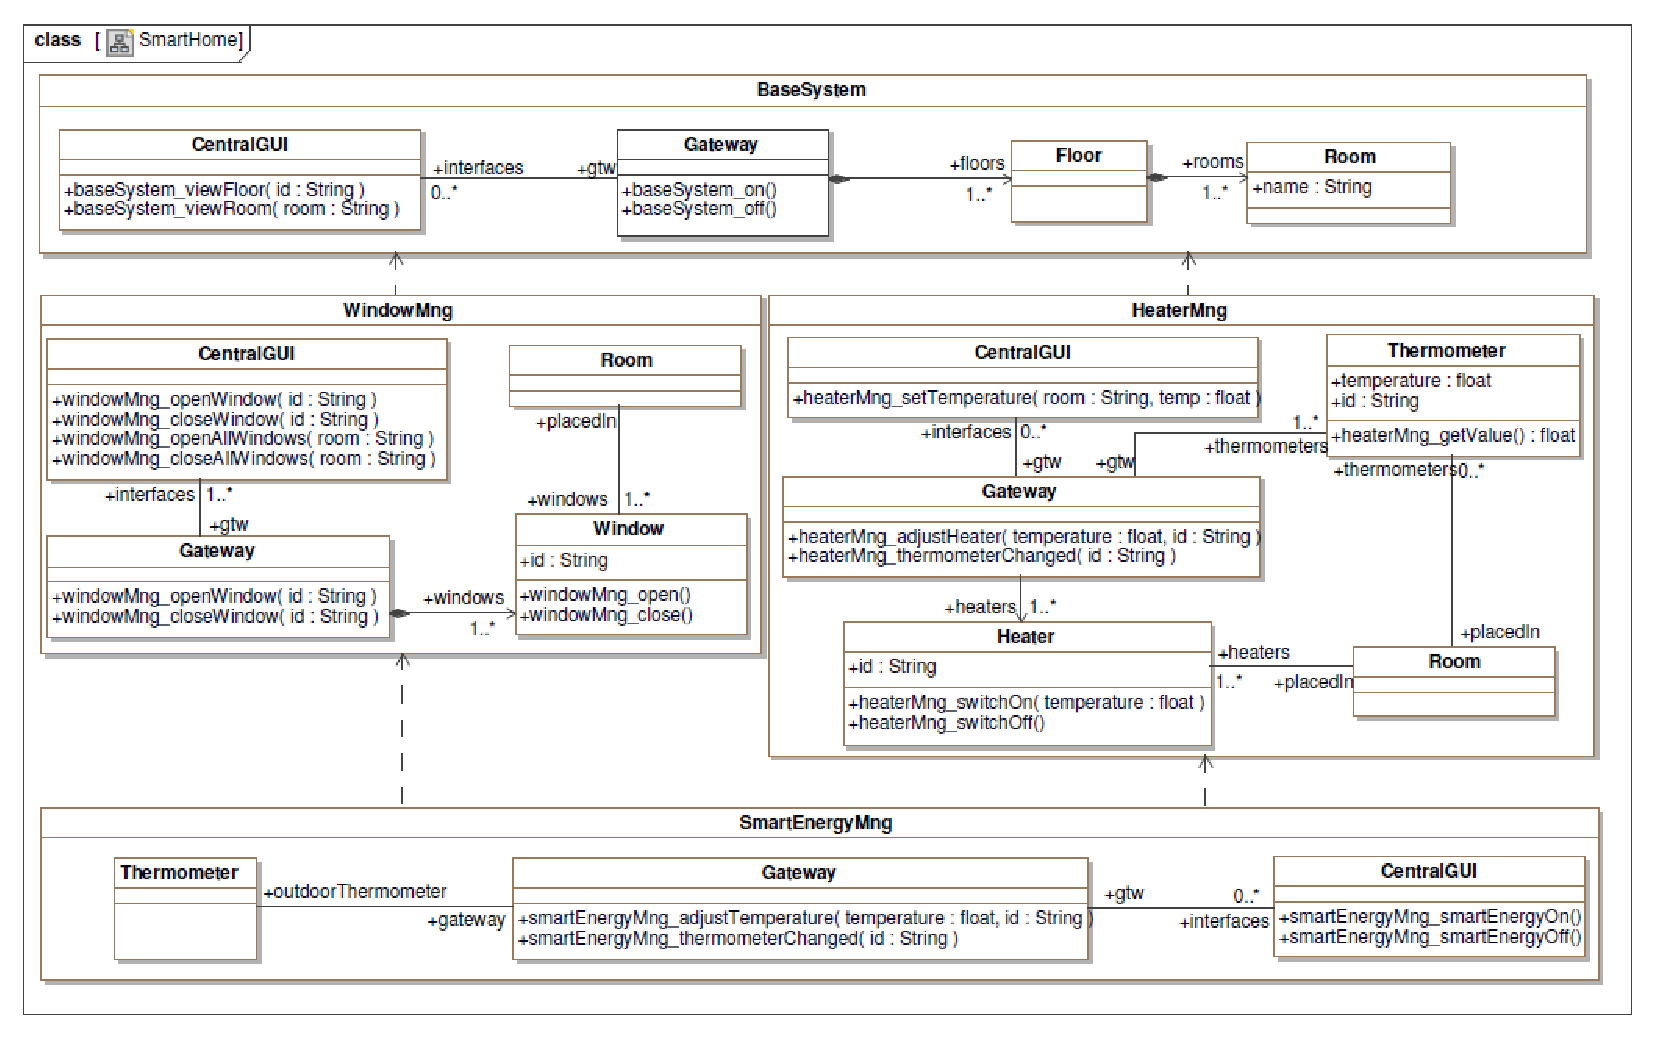
\includegraphics[width=.95\linewidth]{background/images/slicerPattern.eps} \\
  \caption{Proceso de Desarrollo de una L�nea de Productos Software}
  \label{back:fig:slicerPattern}
\end{figure}

Usando esta estrategia se puede comprobar c�mo, por ejemplo, las versiones del m�todo \imp{thermometerChanged} correspondientes a las caracter�sticas \imp{HeaterMng} y \imp{SmartEnergyMng} han sido transformadas en \imp{heaterMng\_thermometerChanged} y \imp{smartEnergyMng\_thermometerChanged} respectivamente y por tanto pueden co-existir sin que sus nombres colisionen. Es m�s, el m�todo \imp{smartEnergyMng\_thermometerChanged} puede extender del m�todo \imp{heaterMng\_thermometerChanged}. Se dispone por tanto de varias versiones parciales de un mismo m�todo. A las versiones prefijadas de un m�todo les denominaremos \emph{versiones sucias} de dicho m�todo.

Para generar un producto espec�fico es necesario que, a nivel de Ingenier�a de Aplicaci�n, se compongan o combinen dichas versiones sucias. Para ello, cada vez que queramos configurar una nueva aplicaci�n, debemos crear, por cada clase que deba ser incluida en el producto final, una nueva clase parcial, la cual se encargar� de combinar o componer dichos m�todos sucios de las clases parciales correspondientes a caracter�sticas. Dicha clase parcial contendr�a lo que denominaremos la \emph{versi�n limpia} de los m�todos a componer, es decir, las versiones de los m�todos sin prefijar, que ser�an adem�s p�blicos.

En nuestro caso, para configurar la clase \emph{Gateway} con control inteligente de la energ�a, se crear�a una nueva clase parcial \emph{Gateway}. Dicho m�todo contendr�a, por ejemplo, el m�todo \imp{thermometerChanged} (sin prefijo alguno).

A continuaci�n, para componer los m�todos, se hace que cada m�todo limpio \emph{delegue} en tantos m�todos sucios como fuere necesario, de acuerdo a las caracter�sticas seleccionadas para el producto que se est� construyendo. En nuestro caso, \imp{thermometerChanged} delegar�a en \imp{smartEnergy\_thermometerChanged}.

Para evitar que los m�todos sucios \imp{heaterMng\_thermometerChanged} y \imp{smartEnergyMng\_thermometerChanged} puedan ser invocados directamente por objetos que no sean de la clase \imp{Gateway}, todas las versiones sucias de un m�todos ser�n privadas. De esta forma, s�lo son invocables las versiones limpias de un m�todo.

Esta idea, tal cual, no puede utilizarse para los constructores de la clases, ya que dichos constructores no se pueden ser renombrados, al tener que seguir un patr�n espec�fico para su nombre. Por tanto, necesitamos utilizar una soluci�n alternativa.

\begin{figure}[tb!]
\begin{center}
\begin{footnotesize}
\begin{verbatim}
File InitialModel/Gateway.cs
--------------------------------------------------------
01 public partial class Gateway {
02      ...
03      private void InitialModel_initGateway() {
04          this.floors = new List<Floors>();
05          this.interfaces = new List<CentralGUI>();
06      }
07 }

File WindowMng/Gateway.cs
--------------------------------------------------------
08 public partial class Gateway {
09      ...
10      private windowMng_initGateway() {
11          this.windows = new List<Window>();
12      }
13 }

File MyHouse/Gateway.cs
--------------------------------------------------------
14 public partial class Gateway {
15      ...
16      public Gateway() {
17          // WindowMng has been selected
18          initialModel_initGateway();
19          windowMng_initGateway();
20      }
21 }
\end{verbatim}
\end{footnotesize}
\end{center}
\caption{\emph{Slicer Pattern} para constructores}
\label{back:code:constSlicerPattern}
\end{figure}


Dicha soluci�n se basa en hacer que la versi�n limpia de un constructor s�lo se cree en el proceso de configuraci�n de un producto software. En las clases parciales \emph{sucias}, en lugar de constructores, tendremos m�todos \emph{especiales}, los cuales contendr�n la l�gica del constructor para dicha clase parcial. De esta forma, cada clase parcial $X$ correspondiente a una caracter�stica $F$ tendr� un m�todo privado llamado $<$F$>$\_init\_$<$X$>$ que contendr� el fragmento de la l�gica del constructor para la clase $X$ correspondiente a la caracter�stica $F$.

La Figura~\ref{back:code:constSlicerPattern} muestra c�mo se aplica dicha t�cnica. Se puede apreciar c�mo la l�gica del constructor para \emph{Gateway} ha sido encapsulada en un m�todo llamado  \imp{initialModel\_initGateway} (Figura~\ref{back:code:constSlicerPattern} l�neas 03-06). Se ha utilizado la misma t�cnica (Figura~\ref{back:code:constSlicerPattern}, l�neas 10-12) para la caracter�stica \imp{WindowMng}. Estos m�todos \emph{init} corresponder�an a la \emph{versi�n sucia} del constructor.

Para componer dichas \emph{versiones sucias} de un constructor de acuerdo a una selecci�n de  caracter�sticas dada, se crea en la clase parcial que representa en producto a configurar el constructor de dicha clase. Dicho constructor constitute la \emph{versi�n limpia} del constructor de la clase. Al igual que en el caso de los m�todos regulares, dicho constructor delegar� en tantos m�todos \emph{init} como sea necesario, de acuerdo a la selecci�n de caracter�sticas realizada.

La Figura~\ref{back:code:constSlicerPattern}, l�neas 16-20, muestra esta soluci�n aplicada al constructor de la clase \emph{Gateway}, entendiendo que s�lo se ha seleccionado como caracter�stica a ser incluida en el producto final \imp{WindowMng}.

Por tanto, a modo de resumen, se puede ver c�mo utilizando el \emph{Slicer Pattern} se pueden extender y sobreescribir m�todos regulares y constructores, solventado las limitaciones inicialmente identificadas de las clases parciales en relaci�n a la implementaci�n de dise�os orientados a caracter�sticas~\citep{sanchez:2010}.

Por tanto, el objetivo de este proyecto es que todo el trabajo que es necesario realizar para instanciar este patr�n, es decir, renombrado de los m�todos para crear las versiones sucias, creaci�n de las versiones limpias correspondientes, as� como del c�digo para delegar en los m�todos que corresponda, sea generado autom�ticamente. Para ello es necesario crear una serie de generadores de c�digo. La siguiente secci�n describe, a grandes rasgos, el funcionamiento de los lenguajes de generaci�n de c�digo.


\section{Generaci�n de C�digo con Epsilon}
\label{sec:back:epsilon}

%%==================================================================%%
%% Author : Abascal Fern�ndez, Patricia                             %%
%%          S�nchez Barreiro, Pablo                                 %%
%% Version: 1.1, 17/04/2013                                         %%
%%                                                                  %%
%% Memoria del Proyecto Fin de Carrera                              %%
%% Background/Generaci�n de C�digo con Epsilon                      %%
%===================================================================%%
Epsilon~\cite{kolovos:2008} es una plataforma para la construcci�n de lenguajes consistentes e interoperables para las tareas de gesti�n de modelado tales como transformaci�n de modelos, generaci�n de c�digo, comparaci�n de modelos, t�cnicas merge, refactorizaci�n y validaci�n. El presente proyecto se ha centrado en la generaci�n de c�digo y por tanto en los lenguajes \emph{Epsilon Generation Language} (EGL) y \emph{Epsilon Object Language}(EOL) proporcionados por Epsilon, que se analizan con m�s detalle a continuaci�n.

\paragraph{Epsilon Generation Language(EGL)} \ \\

EGL es un \emph{plug-in} para Eclipse que proporciona un lenguaje apropiado para las transformaciones modelo a texto (\emph{model-to-text-transformation}, abreviado M2T). EGL puede ser usado para transformar modelos en varios tipos de artefactos de car�cter textual, incluyendo c�digos ejecutables (por ejemplo Java), informes (por ejemplo en HTML), im�genes (por ejemplo usando DOT), especificaciones formales (por ejemplo el lenguaje Z), o incluso aplicaciones completas generadas con m�ltiples lenguajes (por ejemplo HTML, Javascript y CSS).

EGL es un generador de c�digo basado en plantillas; es decir, que la parte programada se asemeja al contenido que se va a generar, proporcionan adem�s diversas caracter�sticas que simplicifan y dan soporte a la generaci�n de texto desde modelos. La figura~\ref{back:fig:epsilonEGL} muestra un ejemplo sencillo del modelo de entrada para un programa EGL, donde se pueden observar tres clases: Persona, Alumno y Profesor. Supongamos que se quiere obtener el nombre de las clases, para ello se deber�a generar un c�digo similar al del listing ~\ref{back:code:generacionClases} donde aparece un bucle (l�neas 1-3) que recorre todas las clases contenidas en el modelo de entrada y en cada una de ellas (l�nea 2) se genera el texto \emph{El modelo contiene la clase: $<$nombre de la clase$>$}. De esta forma el resultado para el ejemplo de la figura~\ref{back:fig:epsilonEGL}, despu�s de haber sido tratado mediante EGL tal como muestra el listing ~\ref{back:code:generacionClases}, queda expuesto en el listing ~\ref{back:code:resultadogeneracionClases}.

\begin{figure}[!tb]
  \centering
	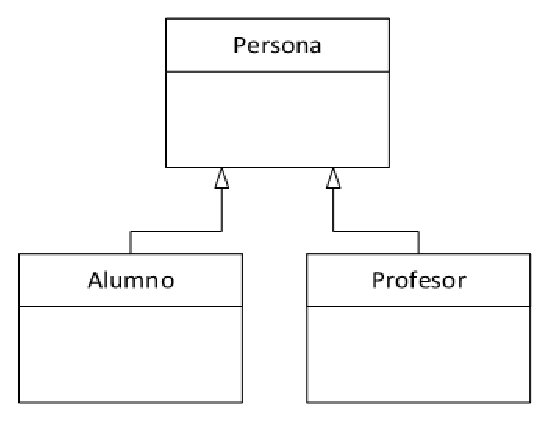
\includegraphics[width=.70\linewidth]{background/images/epsilonEGL} \\
  \caption{Ejemplo de modelo de entrada para generaci�n de c�digo con EGL}
  \label{back:fig:epsilonEGL}
\end{figure}

\begin{lstlisting} [basicstyle=\ttfamily\scriptsize,language=CSharp, captionpos=b,
                    caption=Generaci�n del nombre de cada Class contenida en un modelo de entrada,
                    label=back:code:generacionClases]
1 [% for (c in Class.all) { %]
2     El modelo contiene la clase: [%=c.name%]
3 [% } %]
\end{lstlisting} 

\begin{lstlisting} [basicstyle=\ttfamily\scriptsize,language=CSharp, captionpos=b,
                    caption=Resultado de la generaci�n del nombre de cada Class contenida en un modelo de entrada,
                    label=back:code:resultadogeneracionClases]
1 El modelo contiene la clase: Persona
2 El modelo contiene la clase: Alumno
3 El modelo contiene la clase: Profesor
\end{lstlisting} 

 EGL no solo nos permite generar estos sencillos ejemplos, es una herramienta mucho m�s potente que permite la generaci�n de funciones creadas espec�ficamente por el usuario para facilitar la obtenci�n de datos de los modelos de entrada. Tal como se aprecia en el listing ~\ref{back:code:generacionOperacion} se puede programar una operaci�n que implemente la cabecera de una clase Java y de esta forma invocar dicha funci�n tantas veces como sea necesario en aquellos programas EGL que lo necesiten. En el listing ~\ref{back:code:generacionOperacion} (l�nea 4) la operaci�n \emph{visibility} indica la visibilidad de \emph{self} siendo en este caso la visibilidad de la clase tal como muestra la l�nea 3. Mientras que la operaci�n \emph{name}, al igual que en el listing ~\ref{back:code:generacionClases}, se refiere al nombre del elemento actual, en este caso el nombre de la clase.

\begin{lstlisting} [basicstyle=\ttfamily\scriptsize,language=CSharp, captionpos=b,
                    caption=Uso de una operaci�n que especifica el texto generado para una declaraci�n de una clase Java,
                    label=back:code:generacionOperacion]
1 [%=c.declaration()%]
2 [% @template
3 operation Class declaration() { %]
4     [%=self.visibility] class [%=self.name%] {}
5 [% } %]
\end{lstlisting} 

El tipo Template proporciona tres utilidades b�sicas al usuario:

\begin{enumerate}
	\item  Una Template puede invocar a otras Templates y por tanto pueden ser compartidas y reutilizadas entre programas EGL. En el listing ~\ref{back:code:template} (l�nea 2) se aprecia c�mo desde un programa EGL se llama a otro programa EGL.
    \item El tipo Template permite al usuario definir el destino del texto generado (por ejemplo a una base de datos o ficheros para un proyecto en Visual Studio).  En el listing ~\ref{back:code:template} (l�nea 3) se presenta que el fichero de salida ser� un fichero de extensi�n .txt.
    \item Y por �ltimo, proporciona un conjunto de operaciones que se usan para controlar el destino del texto generado. En el listing ~\ref{back:code:template} (l�nea 3) se muestra c�mo se elige el fichero destino para almacenar el texto generado con la plantilla \emph{ClassNames.egl}.
\end{enumerate}

\begin{lstlisting} [basicstyle=\ttfamily\scriptsize,language=CSharp, captionpos=b,
                    caption=Almacenar el nombre de cada Class en disco,
                    label=back:code:template]
1 [%
2 var t : Template = TemplateFactory.load("ClassNames.egl");
3 t.generate("Output.txt");
4 %]
\end{lstlisting}


\paragraph{Epsilon Object Language(EOL)} \ \\

El principal objetivo de EOL es proporcionar un conjunto rehusable operaciones que son comunes en la gesti�n de modelos. El listing ~\ref{back:code:eol} muestra un ejemplo de operaciones EOL. No es un lenguaje orientado a objetos en el sentido de que no define clases de s� mismo pero sin embargo necesita gestionar objetos de los tipos definidos externamente a el (listing ~\ref{back:code:eol} l�neas 3 y 7, en este caso objetos de tipo Integer). La l�nea 1 del listing ~\ref{back:code:eol} presenta un ejemplo de llamada a operaciones EOL, donde el primer elemento es un 1, de tipo Integer, que llama a la operaci�n add1() y devuelve, tal como se aprecia en la l�nea 4, el valor de \emph{self}+1 es decir 2. A continuaci�n, se vuelve a tomar el valor 2, de tipo Integer, y se realiza la llamada a la operaci�n add2() que devuelve el valor de \emph{self}+2 es decir 4. Y dicho contenido se imprime por pantalla (instrucci�n \emph{println()}).

\begin{lstlisting} [basicstyle=\ttfamily\scriptsize,language=CSharp, captionpos=b,
                    caption=Ejemplo de operaci�n EOL,
                    label=back:code:eol]
1 1.add1().add2().println();
2
3 operation Integer add1() : Integer {
4   return self + 1;
5 }
6
7 operation Integer add2() : Integer {
8   return self + 2;
9 }
\end{lstlisting} 

De esta forma, EOL permite encapsular aquellas operaciones EGL que se vayan a utilizar a lo largo de las respectivas plantillas para evitar la repetici�n innecesaria de c�digo.


\section{Planificaci�n}

%%==================================================================%%
%% NOTA(Pablo): Escribe aqu� una peque�a planificaci�n. Insp�rate   %%
%%              en la del PFC de Tejedo                             %%
%%==================================================================%%

%%==================================================================%%
%% Author : Abascal Fern�ndez, Patricia                             %%
%%          S�nchez Barreiro, Pablo                                 %%
%% Version: 1.2, 18/06/2013                                         %%
%%                                                                  %%
%% Memoria del Proyecto Fin de Carrera                              %%
%% Background/Generaci�n de C�digo con Epsilon                      %%
%===================================================================%%

Como se ha comentado con anterioridad, el objetivo de este Proyecto Fin de Carrera es el desarrollo de una serie de generadores de c�digo que permitan automatizar la aplicaci�n del \emph{Slicer Pattern}. Dichos generadores de c�digo se desarrollar�n utilizando un moderno enfoque de \emph{Ingenier�a de L�neas de Productos Software}. Por tanto, el proceso de desarrollo del presente proyecto queda pr�cticamente determinado por dicho enfoque, el cual posee un proceso de desarrollo bien definido, el cual se describi� en la secci�n~\ref{sec:back:spl}. La Figura~\ref{fig:planning} muestra como dicho proceso de desarrollo se ha instanciado para nuestro caso particular.

\begin{figure}[!tb]
    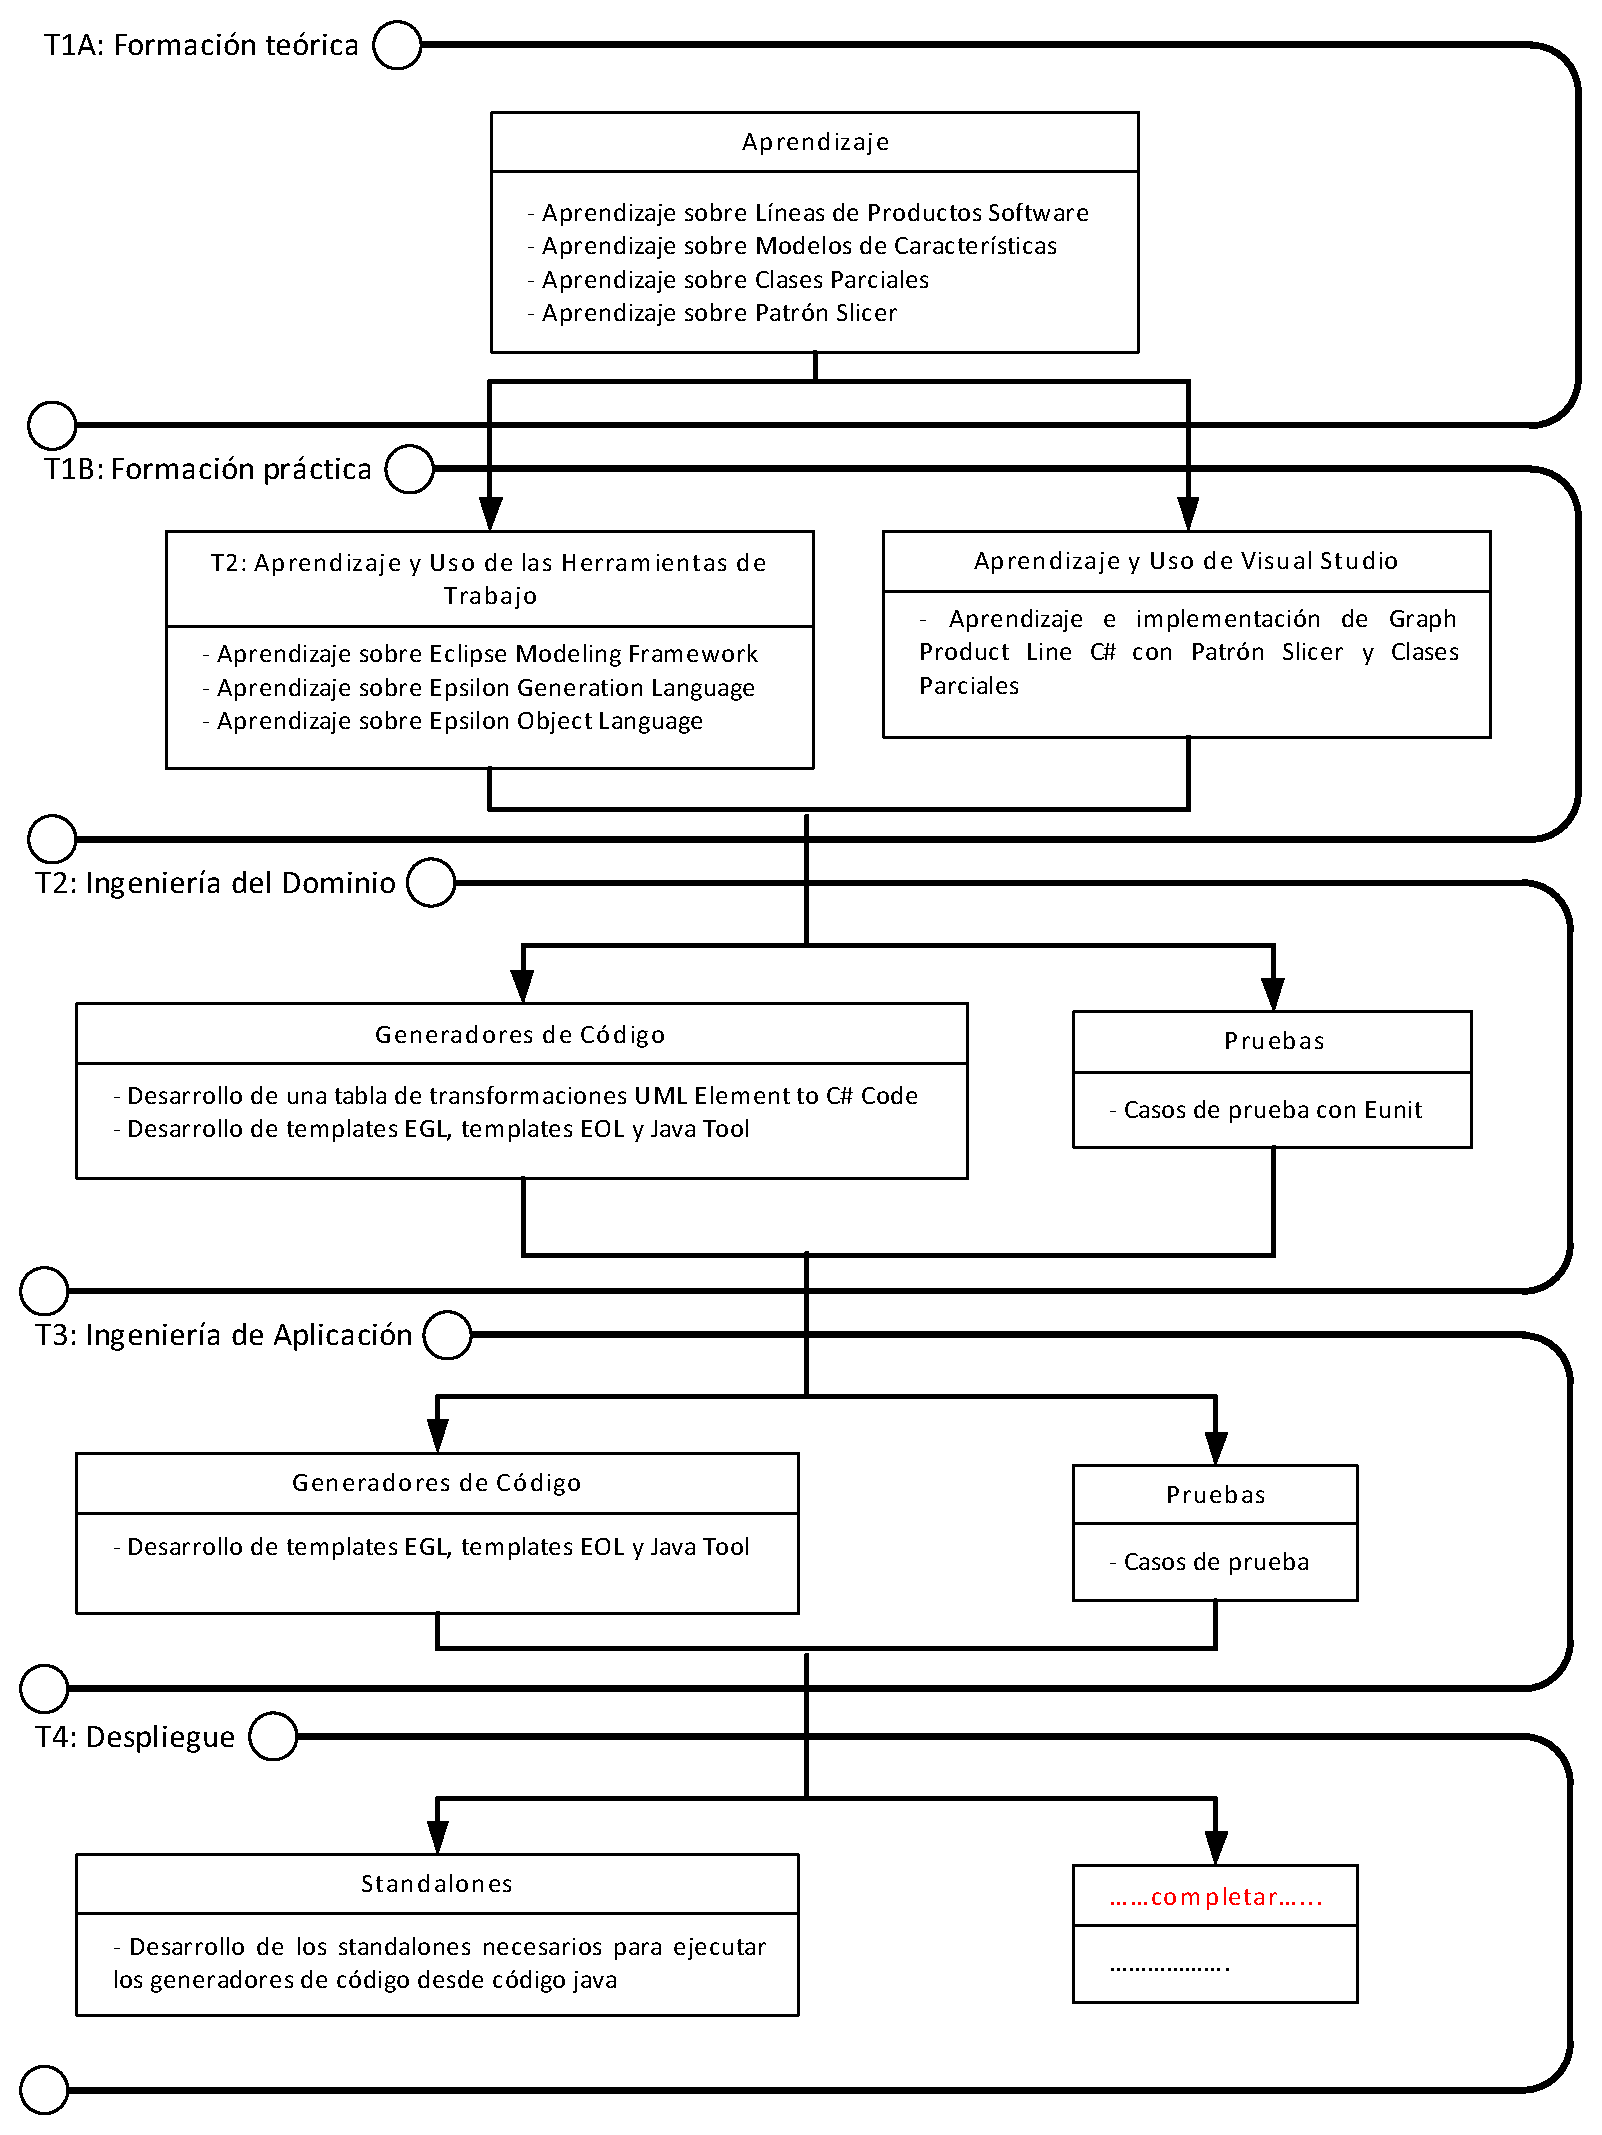
\includegraphics[scale=0.74]{background/images/planning.eps}
    \caption{Proceso de desarrollo del Proyecto Fin de Carrera}
    \label{fig:planning}
\end{figure}

Obviamente, la primera tarea (Figura~\ref{fig:planning}-\emph{T1A} y \emph{T1B}) en este proceso de desarrollo fue la de adquirir los conocimientos necesarios para la realizaci�n de todas las tareas posteriores. Ello implicaba adquirir los conocimientos relacionados con las \emph{L�neas de Producto Software}~\cite{pohl:2010, kakola:2006} en general y con el dise�o orientado a modelos~\cite{kastner:2008}, las clases parciales~\cite{sanchez:2010} y el patr�n slicer ~\cite{perez:2011} en particular.

Dado que el proyecto se deb�a implementar con una herramienta para el desarrollo software dirigido por modelos, denominado \emph{Epsilon}~\cite{kolovos:2008}, el siguiente paso (Figura~\ref{fig:planning}-\emph{T1B} y \emph{T1B}) fue familiarizarse con dicha herramienta y adquirir ciertos conocimientos sobre la utilizaci�n de EMF (\emph{Eclipse Modelling Framework})~\cite{steinberg:2008} para la definici�n de metamodelos y sobre los lenguajes a utilizar para la generaci�n de c�digo, EGL (\emph{Epsilon Generation Language})~\citep{dimitrios:2012} y EOL (\emph{Epsilon Object Language})~\citep{dimitrios:2012}. Adem�s, por exigencias de los usuarios finales de este producto, el c�digo generado deb�a ser editable como un proyecto de Visual Studio 2010, por lo que a continuaci�n se procedi� al manejo y aprendizaje de uso de dicha herramienta mediante la creaci�n de un proyecto de l�nea de productos software aplicando los conceptos te�ricos aprendidos en la etapa \emph{T1A}, es decir las clases parciales C\# y el \emph{Slicer Pattern}.

Tras esta tarea inicial de adquisici�n de conocimientos previos, el resto del proyecto se estructura como un proyecto de Ingenier�a de L�neas de Producto Software. Consecuentemente, la primera tarea tras la fase inicial de documentaci�n (Figura~\ref{fig:planning}-\emph{T2}) fue la fase dedicada a la implementaci�n de la fase de \emph{Ingenier�a del Dominio}, es decir, la implementaci�n de los generadores de c�digo necesarios para transformar el modelo UML dado en un proyecto Visual Studio escrito en lenguaje C\# y que estuviera implementado acorde a las clases parciales C\# y el \emph{Slicer Pattern}, conocimientos adquiridos en la fase \emph{T1} de la planificaci�n. Completando el desarrollo de esta etapa con las pruebas pertinentes mediante el uso de la herramienta EUnit~\citep{dimitrios:2012}.

A continuaci�n, de acuerdo con lo expuesto en la secci�n anterior, procedimos a desarrollar la implementaci�n de la fase de \emph{Ingenier�a de Aplicaci�n} (Figura~\ref{fig:planning}-\emph{T3}) que se desarroll� de manera an�loga a la fase \emph{T2}.

%% %% %% %% %% %% %% %% %% %% %% %% %% %% %% %% %% %% %% %% %% %% %% %% %% %%
\todo{completar con la explicaci�n de la creaci�n del plugin cuando lo termine}
%% %% %% %% %% %% %% %% %% %% %% %% %% %% %% %% %% %% %% %% %% %% %% %% %% %%

En este punto del proceso de desarrollo ten�amos implementado el editor requerido, por lo que s�lo restaba proceder a su despliegue (Figura~\ref{fig:planning}-\emph{T4}). Este despliegue implicaba su integraci�n dentro de la arquitectura de plugins de Eclipse. Tras dicha integraci�n, se procedi� a realizar una serie de pruebas de aceptaci�n, destinadas a comprobar que el trabajo realizado satisfac�a las necesidades de los usuarios finales que iban a utilizar el producto creado.


\section{Sumario}
\label{sec:back:sumario}

%%==================================================================%%
%% Author : Abascal Fern�ndez, Patricia                             %%
%% Author : S�nchez Barreiro, Pablo                                 %%
%% Version: 1.5, 15/05/2013                                         %%
%%                                                                  %%
%% Memoria del Proyecto Fin de Carrera                              %%
%% Application Engineering/Sumario                                  %%
%%==================================================================%%

Este cap�tulo se han descrito la fase de \emph{Ingenier�a de Aplicaci�n} de nuestra l�nea de productos software. Dentro de dicha fase se ha analizado el algoritmo necesario para la generaci�n del producto espec�fico, se ha profundizado tambi�n en el desarrollo e implementaci�n de los generadores de c�digo necesarios para tal fin y sus correspondientes pruebas, por �ltimo se explicado el proceso de empaquetado y distribuci�n del trabajo realizado durante este Proyecto de Fin de Carrera.

